95. а) $|2x-y|=x\Leftrightarrow \begin{cases}\left[\begin{array}{l}2x-y=x,\\2x-y=-x.\end{array}\right.\\x\geqslant0.\end{cases}
\Leftrightarrow \begin{cases}\left[\begin{array}{l}y=x,\\ y=3x.\end{array}\right.\\x\geqslant0.\end{cases}$
$$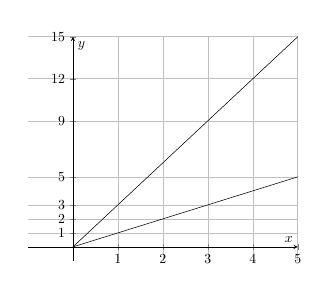
\begin{tikzpicture}[scale=0.5]
\begin{axis}[
    axis lines = middle,
    grid=major,
    legend pos={south west},
    xlabel = {$x$},
    %xlabel style={below right},
    ylabel = {$y$},
    ymin=-1,
    ymax=15,
    xmin=-1,
    xmax=5,
    xtick={ 1,2, 3,4, 5},
    xticklabels={1,2, 3,4, 5},
    ytick={1,2, 3, 5,9,12,15},
    yticklabels={1,2, 3, 5,9,12,15},
                  ]
\addplot[domain=0:5, samples=100, color=black] {x};
\addplot[domain=0:5, samples=100, color=black] {3*x};
        %\addplot[domain=2.01:6, samples=100, color=black] {2/(2-x)};
   % \addplot[domain=-3:3, samples=100, color=black] {-x};
     %\addlegendentry{$\text{Рис. 1}$};
\end{axis}

\end{tikzpicture}$$
б) $|2x-y|<x\Leftrightarrow \begin{cases}2x-y<x,\\ 2x-y>-x.\end{cases}
\Leftrightarrow \begin{cases}y>x,\\ y<3x.\end{cases}$
$$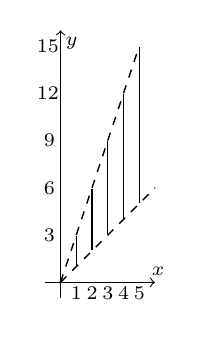
\begin{tikzpicture}[scale=0.2]
\tikzset {line01/.style={line width =0.5pt}}
\tikzset{line02/.style={line width =1pt}}
\tikzset{line03/.style={dashed,line width =0.5pt}}
%\filldraw [black] (0,0) circle (1pt);
\draw [->] (-1,0) -- (6,0);
\draw [->] (0,-1) -- (0,16);
\draw[line01] (1,1.05) -- (1,2.95);
\draw[line01] (2,2.05) -- (2,5.95);
\draw[line01] (3,3.05) -- (3,8.95);
\draw[line01] (4,4.05) -- (4,11.95);
\draw[line01] (5,5.05) -- (5,14.95);
\draw[line03] (0,0) -- (6,6);
%\draw[line01] (-2,-7) -- (-2,7);
\draw[line03] (0,0) -- (5,15);
%\draw[line03] (0,2) -- (1,2);
%\draw[line03] (0,-2) -- (1,-2);
\draw (6.2,0.7) node {\scriptsize $x$};
%\draw (-1.2,-2) node {\scriptsize $-2$};
%\draw (-0.7,2) node {\scriptsize $2$};
\draw (-0.7,6) node {\scriptsize $6$};
\draw (-0.7,3) node {\scriptsize $3$};
\draw (-0.7,9) node {\scriptsize $9$};
\draw (-0.8,12) node {\scriptsize $12$};
\draw (-0.8,15) node {\scriptsize $15$};

\draw (2,-0.7) node {\scriptsize $2$};
\draw (1,-0.7) node {\scriptsize $1$};
\draw (3,-0.7) node {\scriptsize $3$};
\draw (4,-0.7) node {\scriptsize $4$};
\draw (5,-0.7) node {\scriptsize $5$};
%\draw (0.7,-1) node {\tiny $-1$};

%\draw (-2.8,-0.9) node {\tiny $-2$};
\draw (0.7,15.2) node {\scriptsize $y$};
%\draw (1,2) circle (8pt);
%\draw (-2,-3) circle (8pt);
\end{tikzpicture}$$
